\setchapterstyle{kao}
\setchapterpreamble[u]{\margintoc}
\chapter{Neutrinos in High Energy Universe}
\labch{nu_theory_sources}
\begin{figure}[h]
    \caption[Measured and predicted neutrino fluxes from natural sources]{Measured and predicted neutrino fluxes of neutrinos from various sources. Solar neutrinos are neutrinos, while geo-neutrinos and nuclear reactors are antineutrinos. Other sources produce roughly equal numbers of neutrinos and antineutrinos. Neutrinos from the Big Bang, diffuse su- pernova neutrinos, and high-energy cos- mogenic neutrinos remain undetected. Figure from \cite{KATZ2012651}}
    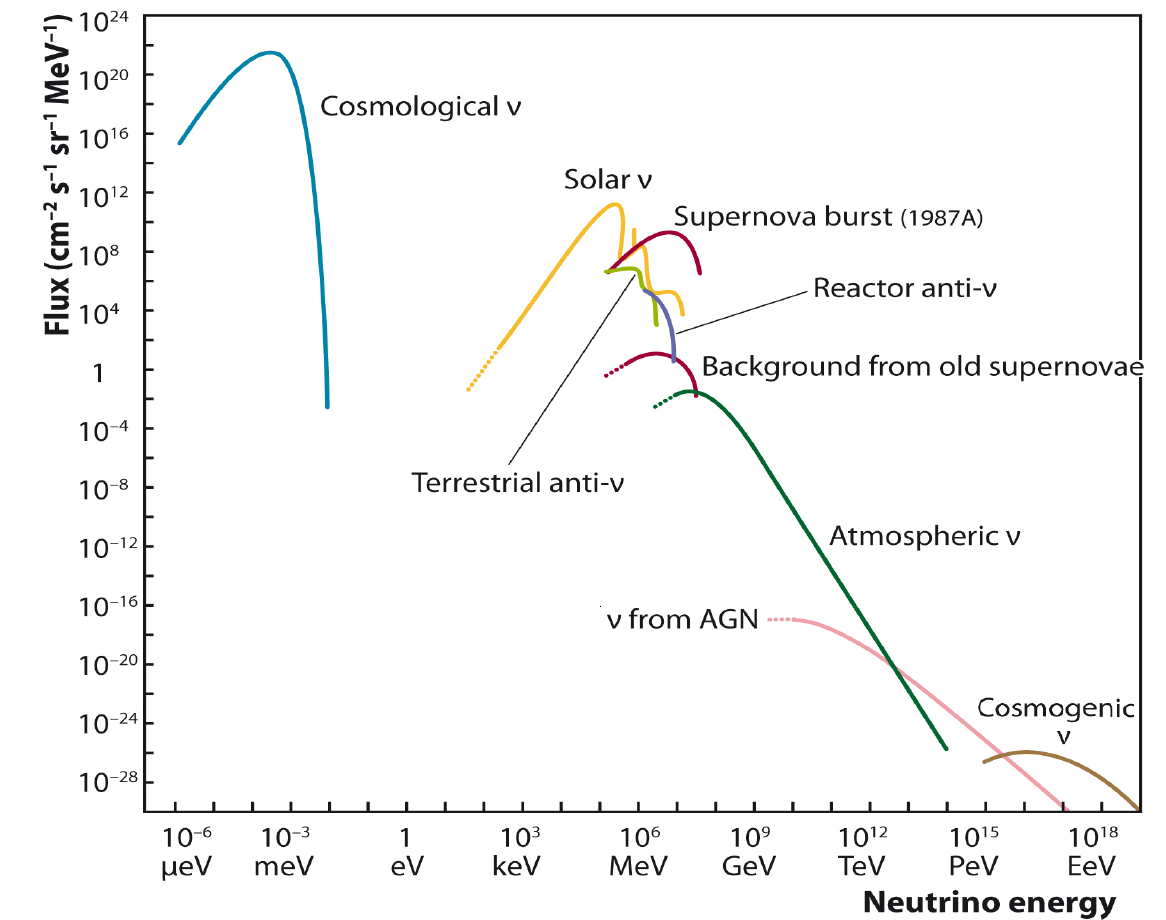
\includegraphics{./figures/nu_phenomenology/all-nu-spectrum-mod.png}
    \labfig{nu_spectrum}
\end{figure}
Neutrinos are produced by various sources across a very large energy range (see \reffig{nu_spectrum}), which include human made sources, such as particle accelerators and nuclear reactors on Earth, and natural sources, such as the atmosphere, sun and other high energy sources from the universe. The largest flux of neutrinos comes from nuclear fusion in the Sun \sidecite{Bahcall} and naturally occurring $\beta$-decay on Earth (the so-called \emph{GeoNeutrinos} or \emph{terrestrial neutrinos}) \sidecite{Krauss}. Historically, a flux of a similar magnitude was briefly observed during the supernova SN1987a in the Large Magellanic Cloud, though it only lasted a few seconds \sidecite{SN1987A_superK,SN1987A_Baksan,SN1987A_IMB}. A more constant, but significantly lower, flux is thought to arise from numerous supernovae throughout the universe \sidecite{Vissani}. High-energy neutrinos, above 1 TeV, originate from either the atmosphere or astrophysical sources, where astrophysical defines galactic and extragalactic origin, and are of a particular interest for the work presented in this thesis. 

As high-energy neutrinos (above tens of TeV) are expected to be produced alongside cosmic rays at high-energy acceleration sites, this chapter will first introduce cosmic rays. It will then cover the production of neutrinos and muons from cosmic ray interactions with the Earth's atmosphere, followed by a discussion on neutrinos generated at cosmic ray acceleration sites.

\section{Cosmic Rays}
\label{sec:cosmic_rays}
Cosmic rays were first discovered by Victor Hess during his famous balloon flight in 1912, where he measured a significant increase in ionization rates as he ascended in altitude \sidecite{HESS_Balloon}. This finding provided the first direct evidence for the existence of highly energetic particles arriving from outer space. Over a century later, cosmic ray research has evolved, and today various experiments routinely measure their physical properties. Cosmic rays are now understood to consist mainly of ionized atomic nuclei, with electrons contributing minimally due to significant energy losses during their propagation. Approximately 90\% of cosmic rays are protons, 9\% are helium nuclei ($\alpha$-particles), and the remaining fraction consists of heavier nuclei such as carbon, oxygen, and iron \sidecite{PDG2022}. The primary composition of cosmic rays depends on energy, shifting from light nuclei to heavier nuclei and then back to lighter nuclei as energy increases. However, results from various measurements diverge, making this a highly active area of research. 

Cosmic radiation that reaches the Earth's atmosphere contains all stable charged particles and atomic nuclei with lifetimes of $10^6$ years or more. These particles are divided into \emph{primary} and \emph{secondary} cosmic rays. Primary cosmic rays are particles that are directly accelerated by astrophysical sources. These include protons, helium nuclei, and heavier elements formed in stars. On the other hand, secondary cosmic rays are produced when primary cosmic rays interact with interstellar matter. For example, when primary cosmic rays  collide with gas particles in space, they can create lighter elements like lithium, beryllium, and boron, which are not typically formed in stars. These secondary particles help scientists understand the interactions cosmic rays experience as they travel through the galaxy \sidecite{PDG2022}.

\begin{figure}[h]
    \caption[The all-particle cosmic-ray flux as a function of the energy per nucleus]{The all-particle spectrum as a function of E (energy-per-nucleus) from air shower measurements. The various features of the spectrum discussed in the text are marked with \emph{Knee, 2nd Knee and Ankle}. Data points are referenced in \cite{PDG2022}}
    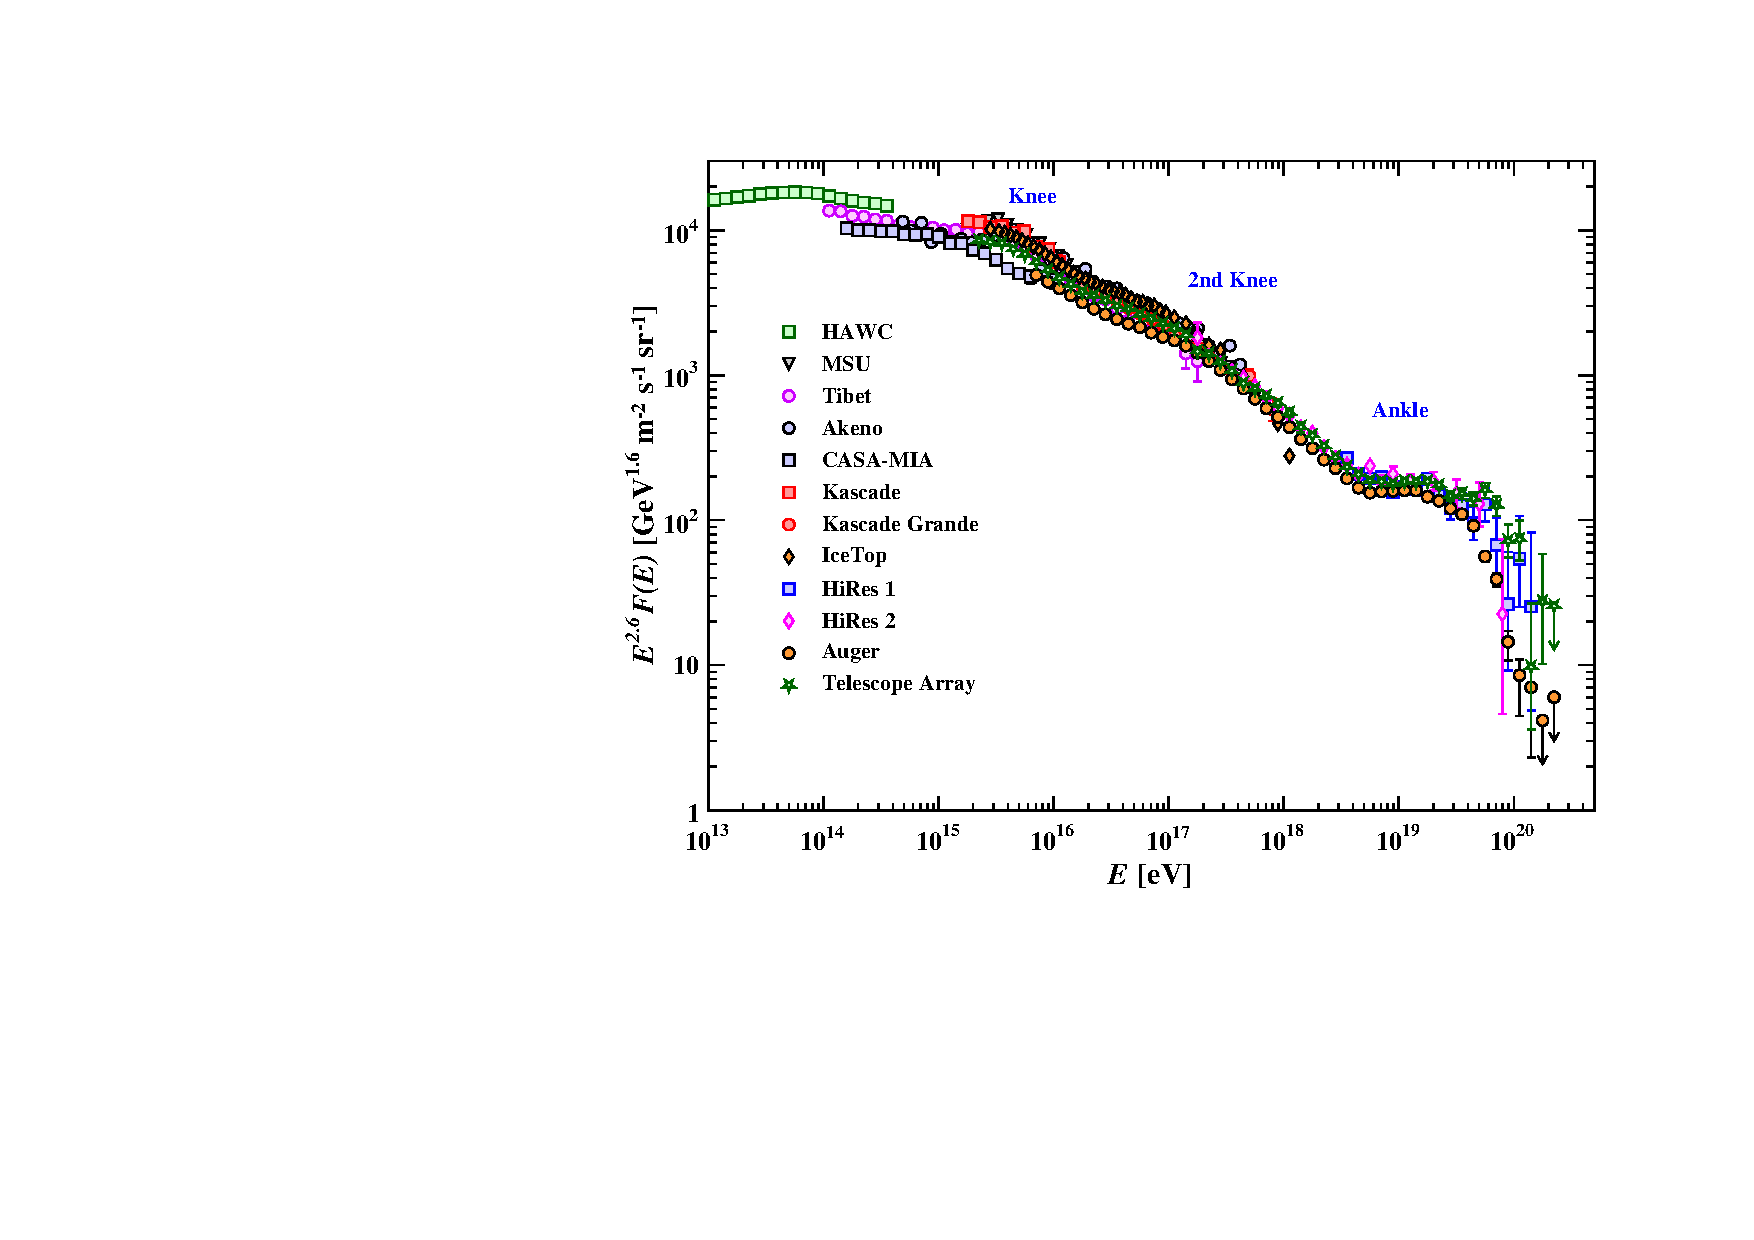
\includegraphics{./figures/nu_he/cr_fig8_AllParticle_21.pdf}
    \labfig{cosmicray_spectrum}
\end{figure}

The energy spectrum of cosmic rays as shown in \reffig{cosmicray_spectrum} is one of their most fascinating characteristics.. The spectrum follows a power-law distribution, expressed as:

\begin{equation}\label{eq:flux}
\frac{dN}{dE} \propto E^{-\gamma}
\end{equation}


where \( E \) is the energy and \( \gamma \) is the spectral index. This form of the spectrum indicates that cosmic rays are accelerated by non-thermal processes, such as shock waves or magnetic reconnection. The spectral index \( \gamma \) is not constant across all energies but changes at specific points in the spectrum (as indicated in \reffig{cosmicray_spectrum}), indicating transitions between different source classes or acceleration mechanisms. Over a vast energy range (from $\sim10^9 \, \mathrm{eV} \, \mathrm{to} \, \sim 10^{15} $), the differential flux given in Equation~\ref{eq:flux} follows a power law with index $\gamma\approx2.7$. The flux in this range is large enough to be directly measured by space and balloon experiments before they interact in the atmosphere \sidecite{ATIC,AMS02,CREAM}.

\marginnote{\begin{kaobox}
    The various features \cite{PDG2022} that can be seen in the \reffig{cosmicray_spectrum} using Equation~\ref{eq:flux} are as follows:
    \begin{equation*}
        \frac{dN}{dE} \sim
            \begin{cases}
            E^{-2.7} & \text{(up to knee)}\\ 
            E^{-3.1} & \text{(knee) }  \\
            E^{-3.3} & \text{(second knee)} , \\
            E^{-2.5} & \text{(ankle)}
            \end{cases}
    \end{equation*}
\end{kaobox}} 

At higher energies, where the cosmic ray flux is too low to be measured directly, they can only be observed indirectly through the cascade of secondary particles they produce in the atmosphere. The energy and type of the primary cosmic ray must then be estimated based on the characteristics of this particle shower. The first significant feature in the cosmic ray energy spectrum is known as \textbf{the knee}, which occurs at an energy of about 3 PeV. At this point, the spectrum softens, with the spectral index \( \gamma \) increasing from around 2.7 to about 3.1. A milder, \textbf{second knee} occurs at around \( 10^{17} \, \text{eV} \) (100 PeV), where the spectrum softens further to $\gamma\sim3.3$.  The Cosmic rays above \( \sim10^{18} \, \text{eV} \) are called \textbf{Ultra High Energy Cosmic Rays (UHECRs)}. At these ultra high energies, the spectrum undergoes a hardening at around \( 10^{18} \, \text{eV} \), where the index returns to a value closer to 2.5. This feature of the spectrum is known as \textbf{ankle} \sidecite{H_RANDEL_2007}. At the highest energies, specifically beyond \(10^{18}\) eV, a decline in cosmic ray flux is expected. This decrease can be explained by \textbf{the Greisen-Zatsepin-Kuzmin (GZK)} mechanism, which involves the production of pions through photohadronic interactions between high-energy protons (E$\sim$50 EeV ($50\times10^{18}$ eV)) and photons from the cosmic microwave background (CMB) \sidecite{GZK1,GZK2}. For this GZK effect to fully account for the observed spectral cutoff, a proton-only composition is necessary. However, data from the Pierre Auger Observatory (PAO) and the Telescope Array (TA) suggest otherwise, indicating a more mixed composition \sidecite{Ankle_AugerPaper,auger_ta_joint}. Another possible explanation for the observed flux suppression is the finite maximum energy that cosmic ray sources can accelerate particles to \sidecite{Das_2021}.

These transitions in the spectrum are believed to be associated with changes in the source population. The initial segment of the cosmic ray energy spectrum, extending up to the knee can largely be explained by the process of particle acceleration occurring within Galactic sources, predominantly supernova remnants \sidecite{modelling}. Supernova remnants serve as dynamic environments where powerful shock waves are generated following the explosive death of massive stars. These shock waves facilitate the acceleration of particles, including protons, to high energies through mechanisms such as Fermi acceleration (see below) \sidecite{Perkins}. The steepening of the spectrum at the knee suggests that accelerators may have reached their maximum capacity for proton acceleration  \sidecite{H_randel_2003}. This limit depends largely on the strength of magnetic fields in the acceleration region, which are crucial for confining charged particles and facilitating energy gain. Additionally, cosmic ray leakage from the Galaxy can reduce high-energy cosmic rays through interactions with interstellar medium particles, contributing to the observed changes in the energy spectrum \sidecite{somthingCR}. 

The second knee in the cosmic ray spectrum can also be understood using similar principles. This feature may arise from the behavior of heavier elements, which experience different acceleration dynamics compared to protons \sidecite{H_randel_2003}. These heavy nuclei may encounter limitations in their acceleration processes, preventing them from reaching energies comparable to lighter particles. Moreover, just like protons, these heavier elements may also face barriers that inhibit their escape from the Galactic environment. Consequently, the second knee could signify a threshold beyond which heavier cosmic rays cannot be further accelerated or are unable to exit the Galaxy, leading to a corresponding steepening in the spectrum. Overall, these observations underscore the complex interplay between magnetic field strengths,  acceleration mechanisms, and propagation effects that shape the cosmic ray energy spectrum. Regarding the ankle region, several proposed models that seek to explain this phenomenon suggest a transition in the primary component from galactic sources to extragalactic ones \sidecite{ankle1,ankle2,ankle3}.

Anisotropies in the arrival directions of cosmic rays (CRs) offer crucial insights into their origins. Identifying these sources becomes theoretically possible if the properties of cosmic ray particles, as well as galactic and extragalactic magnetic fields, are sufficiently well understood. The Pierre Auger Observatory has identified a large-scale dipolar anisotropy in cosmic rays with energies above 8 EeV, with a significance of $6.9\sigma$. The amplitude of this dipole is $d = 0.073^{+0.010}_{-0.008}$, and its direction is approximately $115^\circ$ away from the Galactic Center, supporting the extragalactic origin of UHECRs beyond this energy threshold \sidecite{anisotropy_PAO}. These findings align with results obtained by combining the data from both the Pierre Auger Observatory and the Telescope Array (TA) \sidecite{anisotropy_TA}.

\subsection{Acceleration Mechanism}
\label{sec:accln}
Even during the most powerful solar flares, the Sun is limited to accelerating particles to around 1 GeV \sidecite{solar_flare}. This limitation leads to the question of how cosmic rays can be accelerated to much higher energies, ranging from tens of GeV up to 100 EeV, and what astrophysical sources and mechanisms are responsible for such acceleration. One leading theory, initially proposed by Enrico Fermi, is that cosmic ray particles gain energy through random scattering across moving shock fronts, a process known as first-order Fermi acceleration \sidecite{fermi_accln}. In this process, the relative energy gain $\Delta E$ for a particle with energy $E$ during each scattering event is proportional to the shock velocity $u$, expressed by the equation:

\begin{equation}
    \frac{\Delta E}{E} \sim \frac{u}{c},
\end{equation}

where $c$ is the speed of light \sidecite{Gaisser_Engel_Resconi_2016}. \sidenote{For instance, supernova remnants, where the shock front velocity $u/c \gtrsim 10^{-2}$, create a highly efficient environment for particle acceleration.} A charged particle, starting in the unshocked region, moves into the shocked medium and experiences elastic scattering from magnetic irregularities. With every crossing of the shock front, the particle gains more energy. After $n$ cycles, the particle's energy is given by $E_n = E_0(1 + \alpha)^n$, where $E_0$ is its initial energy and $\alpha$ represents the fractional energy increase per cycle, approximately $\alpha \approx 4v/3c$ \sidecite{Gaisser_Engel_Resconi_2016}. However, particles cannot remain in the shock zone indefinitely, as they may either just loose the energy or \emph{escape} the region. The latter is determined by their escape probability, $p_{\text{esc}} = 4(u - v)/c$, which increases as the shock slows down relative to the surrounding medium.

The resulting energy spectrum of the accelerated particles typically follows a power law, with the differential energy distribution given by $dN/dE \propto E^{-\gamma}$, where $\gamma \approx 1 + \frac{p_{\text{esc}}}{\alpha}$ \sidecite{Perkins}. In non-relativistic shocks moving faster than the speed of sound in the medium, this leads to a spectral index of approximately $\gamma \approx 2.1$. The steeper cosmic ray spectrum, approximately $\sim E^{-2.7}$\sidenote{Although, it is worth to note that it is the \emph{observed} spectrum that steepens due to the diffusion, while the production spectra at the sources can still be approximated by $\gamma\approx2.1$}, can be explained by energy-dependent diffusion in galactic magnetic fields \sidecite{Batista_2014,Snodin:2015fza}.

Although first-order Fermi acceleration is a strong model for non-relativistic shocks, other mechanisms have been proposed to account for even higher-energy particles. These include relativistic shock fronts \sidecite{1987ApJ,1988MNRAS}, where shocks travel close to the speed of light, as well as processes like magnetic reconnection \sidecite{RevModPhys.82.603}, where energy is released when magnetic fields reconfigure, and plasma wakefield acceleration \sidecite{Chang:2007um}, where particles are accelerated by intense electric fields in plasmas. Such processes are crucial in extreme astrophysical environments like active galactic nuclei (AGN) and gamma-ray bursts (GRBs), where cosmic rays are believed to be accelerated to ultra-high energies.

\subsection{Sources}
\label{sec:cosmic_sources}
The notion of Fermi acceleration, as explained in Section~\ref{sec:accln}, fundamentally relies on the confinement of cosmic rays, which allows them to engage in repeated interactions with a shock front or other magnetized structures. If we assume that this confinement is provided by a magnetic field of strength \(B\), it follows that the size of the confinement region, denoted as \(r\), must be greater than the gyro-radius of the cosmic ray. This relationship is described by the following inequality:

\begin{equation}
    r > \frac{E}{ZBc}
\end{equation}

Here, \(E\) represents the energy and \(Z\) is the charge of the cosmic ray, which we typically consider to be ultra-relativistic. Alternatively, this condition can be reformulated as a constraint on the rigidity \(R\), defined as the ratio of the particle's momentum to its charge:

\begin{equation}
    R = \frac{E}{Z} < Bcr.
\end{equation}

\begin{figure}[h]
    \caption[Hillas diagram]{Hillas diagram illustrating different candidate source classes of cos- mic rays. Figure from \cite{hillas_plot}}
    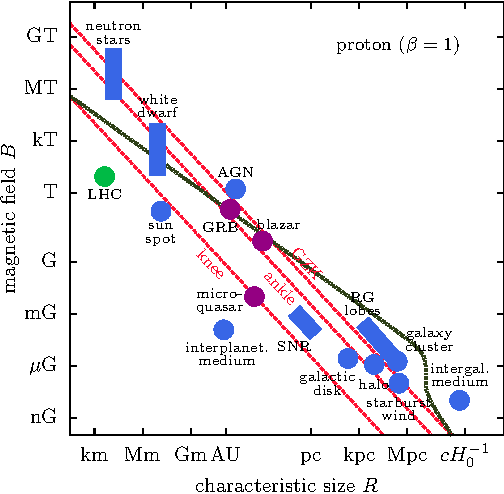
\includegraphics{./figures/nu_he/Hillas_simple.pdf}
    \labfig{hillas}
\end{figure}

This limitation is referred to as \textbf{the Hillas criterion} \sidecite{hillas}. By employing estimates for the sizes and magnetic field strengths of various astronomical objects, one can identify potential sites for acceleration that align with specific cosmic-ray rigidities. The Hillas diagram as shown in \reffig{hillas}, effectively illustrates the magnetic field strength and sizes of different classes of objects.

Following the aforementioned concept, Hillas proposed a simple model that captures the characteristics observed in the energy spectrum and composition of cosmic rays. In this framework, the diagonal lines in \reffig{hillas} signify thresholds below which a source cannot confine a particle with energy \(E\) and charge \(Z\). Considering that the Milky Way has a thickness of no more than 1 kpc \sidecite{Rix:2013bi} and its magnetic field strength is approximately a few $\mu G$ \sidecite{Haverkorn:2014jka}, the Hillas diagram suggests that UHECRs must originate from extragalactic sources. Conversely, galactic supernova remnants (SNRs) emerge as strong candidates for the source of low-energy cosmic rays. While the exact rate of galactic supernova occurrences remains somewhat uncertain, a conversion of just a few percent of the shock wave's energy into particle acceleration would adequately explain the observed cosmic ray flux  below the knee of the cosmic ray spectrum \sidecite{Perkins}.

The origins of cosmic rays in the intermediate energy range (between the second knee and the ankle) are still not fully understood \sidecite{Halzen:2010yj}. Their acceleration is thought to take place within vast magnetic fields generated by substantial bulk flows of relativistic charged particles, which are driven by immense gravitational forces present in the vicinity of neutron stars or black holes. Some plausible candidates for these highest-energy cosmic rays include \textbf{Active Galactic Nuclei (AGN)} \sidecite{Protheroe:1992qs} and \textbf{Gamma-Ray Bursts (GRB)} \sidecite{Wang:2007xj}. 

Active galactic nuclei are extremely bright and compact regions located at the centers of galaxies, powered by supermassive black holes. In these regions, the \emph{infalling} matter forms an accretion disk, where gravitational energy is converted into electromagnetic energy, resulting in the emission of a wide spectrum of radiation (specially when viewed from different directions), from radio waves to gamma rays \sidecite[-8cm]{AGN_picture}. The intense gravitational pull of the black hole compresses the surrounding material, generating high temperatures and pressures. Some AGNs also produce relativistic jets, which are streams of charged particles moving at speeds close to the speed of light. These jets can terminate in hot spots or lobes, providing an environment capable of accelerating cosmic rays to energies nearing 100 EeV \sidecite{Peterson_1997}. 

Gamma-ray bursts, on the other hand, are extremely luminous and transient events characterized by their emission of gamma radiation for brief periods, ranging from milliseconds to several minutes. During their short duration, GRBs emit more energy than any other steady gamma-ray source in the universe \cite{AGN_picture}. A typical GRB bolometric luminosities are of the order of $10^{51} \,\frac{\text{erg}}{\text{s}}$ \sidecite{GRB_lumino}. Theoretical models describing GRBs, such as the fireball shock model \sidecite{PIRAN1999575}, predict an initial short burst of highly energetic gamma rays followed by a more prolonged afterglow that emits across a broad range of wavelengths, from X-rays to radio frequencies. Long GRBs, which last over 2 seconds, are generally believed to be associated with the core collapse of a massive progenitor star \sidecite{hjorth2011gammarayburstsupernova}. In contrast, shorter GRBs are likely the result of the merger of two neutron stars or a neutron star with a black hole \sidecite{LIGOScientific:2017zic, Janka:1999qu}. In both scenarios, the collapse produces highly relativistic jets that exhibit multiple shock fronts, facilitating the acceleration of cosmic rays to extreme energies.


\section{High Energy Neutrinos}
\label{sec:cosmic_nu}
High energy neutrinos are high-energy neutrinos produced through various mechanisms. \textbf{Astrophysical neutrinos} are produced in hadronic interactions within extreme environments like active galactic nuclei and gamma-ray bursts, often in conjunction with cosmic rays. \textbf{Cosmogenic neutrinos} on the other hand, are the neutrinos produced in high energy acceleration cites where UHECRs come from. Lastly, \textbf{Atmospheric neutrinos} are produced when cosmic rays collide with Earth's atmosphere, initiating air showers that generate mesons like pions and kaons. These mesons decay, leading to the production of neutrinos, along with muons and electromagnetic cascades. 

\begin{marginfigure}
    \caption[Schematic of extensive air shower]{Schematic of progress of a particle cascade when a cosmic ray proton interacts with a nucleus in atmosphere. Figure adapted from \cite{CR_shower_fig}.}
    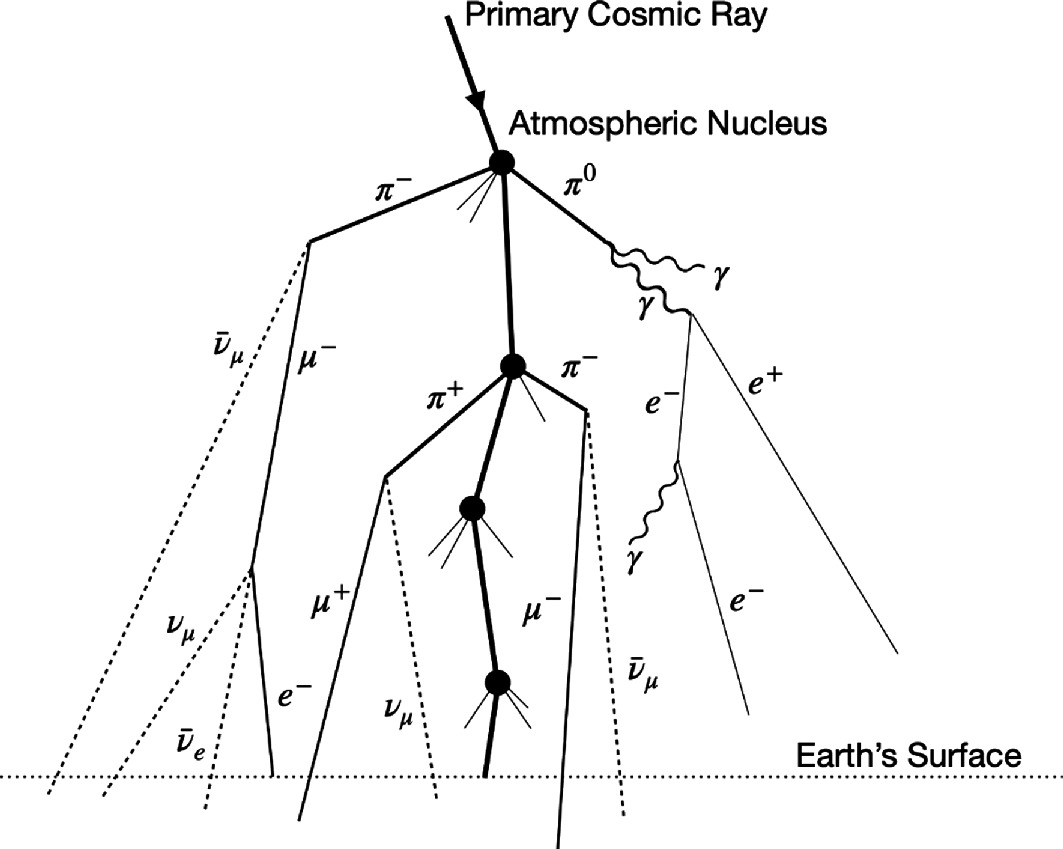
\includegraphics{./figures/nu_he/CRshower.png}
    \labfig{shower}
\end{marginfigure}
Regardless of the source, the basic mechanism of neutrino production of all of the aforementioned neutrinos remains the same, hadronic interactions that produces mesons. The following sections will focus on these neutrino categories, with an emphasis on Astrophysical neutrinos and their production mechanisms, which are most relevant to this thesis.

\subsection{Atmospheric Neutrinos}
\label{sec:atm_nu}
Extensive air showers (EAS) are cascades of secondary particles initiated when a high-energy primary cosmic ray—such as a proton, neutron, or heavier nucleus—interacts with the Earth's atmosphere. These showers can result from cosmic rays with energies reaching \( E \sim 1 \, \text{PeV} \) and beyond, spreading across areas of approximately 10 km² at ground level \sidecite{Gaisser_2012}. When the cosmic ray collides with atmospheric nuclei, it produces a large number of secondary particles, primarily charged and neutral pions (\(\pi^\pm, \pi^0\)), along with kaons (\(K^\pm, K^0\)) and other mesons. A schematic of such a shower development is shown in \reffig{shower}.

The dominant fraction of particles in an EAS consists of pions \sidecite{PDG_2024}. Neutral pions (\(\pi^0\)) decay rapidly into photons (\(\pi^0 \rightarrow 2\gamma\)), feeding the electromagnetic component of the shower, which can be observed through detection techniques such as radio emission \sidecite{LOFAR,AERA}, air fluorescence \sidecite{Auger_fluro}, Cherenkov light \sidecite{auger_cherenkov} and scintillation \sidecite{Abu_Zayyad_2012}. Charged pions (\(\pi^\pm\)) decay into muons and neutrinos. These muons often reach the Earth's surface, where they can be detected by large arrays of particle detectors. If the muons have sufficiently high energy, they can penetrate deep into the ground \sidecite{muon_penetration}, allowing detection by underground observatories like IceCube \sidecite{atm_mu_icecube}. 



The energy spectrum of atmospheric neutrinos can be divided into two main categories: conventional and prompt neutrinos. \textbf{The Conventional Atmospheric Neutrinos} are predominantly produced by the decay of charged pions (\(\pi^\pm\)) and kaons (\(K^\pm\)), which are generated in extensive air showers resulting from cosmic-ray interactions with the Earth's atmosphere (see Equation~\ref{eq:}). The dominant decay channels contributing to the conventional neutrino flux are:\marginnote{\begin{kaobox}
    $K_L^0$ here refers to long-lived neutral kaon which differes from short lived neutral kaon ($K_S^0$) by lifetime and also through decay modes \cite{PDG_2024}. 
\end{kaobox}}
\begin{equation}
    \begin{aligned}
    \pi^\mp &\rightarrow \mu^\mp + \barp{\nu_\mu}, \\
    K^\mp &\rightarrow \mu^\mp + \barp{\nu_\mu}, \\
    K^\mp &\rightarrow \pi^0 + e^\mp + \barp{\nu_e}, \\
    K_L^0 &\rightarrow \pi^\pm + e^\mp + \barp{\nu_e}.
    \end{aligned}
\end{equation}
    
At lower energies (a few GeV), the muons produced in pion and kaon decays usually decay in the atmosphere, leading to an observed flavour ratio of \(\nu_e : \nu_\mu \approx 1:2\). However, at higher energies (above 100 GeV), most muons reach the ground before decaying, significantly reducing the production of electron-neutrinos and causing the flavour ratio to drop below \(1:10\) at TeV energies. This energy-dependent behavior is a key characteristic of the conventional neutrino flux, which dominates in the GeV to TeV range and follows a power law of \(E^{-3.7}\) \sidecite{PDG_2024}. At energies well above 100 GeV, the contribution of charged pions to the muon-neutrino flux diminishes, and kaon decays become the predominant source of conventional atmospheric neutrinos. Due to the differing decay channels and branching ratios, muon-neutrinos (\(\nu_\mu\)) are produced in much higher numbers compared to electron-neutrinos (\(\nu_e\)), with the flavour ratio \(\nu_\mu : \nu_e\) varying between 20:1 to 30:1 in the TeV to PeV range. 

\marginnote{\begin{kaobox}
    The production of prompt atmospheric tau-neutrinos is highly suppressed and is expected to occur primarily through the decay channel \( D_s^\mp \rightarrow \tau^\mp + \barp{\nu_\tau} \), followed by the subsequent decay of the tau lepton \( \tau^{-} \rightarrow \mu^{-} + \bar{\nu_\mu} + \nu_\tau \) \cite{prompt_tau}. The contribution of tau-neutrinos to the overall prompt neutrino flux is approximately 5\% and is generally considered negligible.
\end{kaobox}}

In contrast, \textbf{The Prompt Atmospheric Neutrinos} originate from the rapid decay of charmed mesons (such as \(D^\pm, D^0, D_s^\pm\)), which decay almost immediately after their production without significant interaction. These mesons decay into both muon- and electron-neutrinos via the processes: 
\begin{equation}
    D^\mp \rightarrow \l^\mp + \barp{\nu_l} + X , \quad D^0 \rightarrow l^\pm + \nu_l +X ,
\end{equation}
where, X stands for \emph{anything} in the inclusive decay mode. The aforementioned decay leads to an expected flavour ratio of \(\nu_\mu : \nu_e \approx 1:1\) for prompt neutrinos. The prompt neutrino flux follows the energy distribution of the primary cosmic ray and is unaffected by atmospheric density. 

The energy spectrum of the conventional atmospheric neutrino flux has been measured up to several hundred GeV by underground experiments like Super-Kamiokande \sidecite[-1cm]{superk_atmflux} and the Fréjus Nucleon-Decay Detector \sidecite{Frejus_ref}, and up to a few hundred TeV by IceCube \sidecite{icecube_nue} and ANTARES \sidecite{antares_atmnu}. However, a prompt atmospheric neutrino flux remains undetected, as the predicted normalization lies below the current detection threshold \sidecite{prompt_tau}. Efforts are underway to combine data samples to improve sensitivity and potentially observe this elusive flux \sidecite{icecube_prompt}. Additionally, IceCube has successfully measured atmospheric muon fluxes up to energies of 1 PeV \sidecite{atm_mu_icecube}. The steeper spectrum of conventional neutrinos arises from the fact that charged pions and kaons interact several times before decaying, particularly at higher energies. By contrast, prompt neutrinos, produced directly from the decay of charmed mesons without prior interaction, retain an energy distribution similar to that of the primary cosmic ray. The prompt neutrino flux is also independent of zenith angle, whereas the conventional neutrino flux is most pronounced for neutrinos coming from the horizon, due to the increased probability of pion and kaon decay over longer travel distances through the atmosphere.


\subsection{Cosmogenic Neutrinos}
\label{sec:cosmogenic_nu}
Ultra-high-energy cosmic rays (UHECRs) interact with the cosmic microwave background (CMB) during propagation, generating a flux of neutrinos above PeV energies. The neutrinos at this high energy are known as \textbf{The Cosmogenic Neutrinos}. Given the low flux of UHECRs \sidecite{PDG_2024}, cosmogenic neutrinos are expected to have a flux lower than that of astrophysical neutrinos, though the exact reduction depends on the UHECR composition, spectrum, and source evolution \sidecite{AHLERS2015392}. Detecting or constraining this flux enables us to indirectly test models of UHECR production and composition, where a high cosmogenic neutrino flux would imply a light, proton-dominated composition, and a low flux would suggest a heavier composition \sidecite{Aloisio:2015ega}.

For a pure-proton UHECR composition, the ankle feature can be explained by \emph{the dip model} \sidecite{Berezinsky:2002nc} while the cutoff at \(5 \times 10^{19} \, \text{eV}\) aligns with the GZK effect \sidecite{GZK1,GZK2}; a heavy composition instead implies that the cutoff results from an acceleration limit at the source. Current IceCube limits (5 PeV–50 EeV) mostly rule out a pure-proton scenario, favoring a heavier UHECR composition at the highest energies \sidecite{IceCube:2016uab}. While no significant observations have been made yet of these cosmogenic neutrinos, the radio detection technique, that targets detection of $\sim$ EeV scale neutrinos using \emph{Askaryan effect} \sidecite{Askaryan}, shall be able to help overcome this barrier \sidecite{whitepaper, rnog}. 

\subsection{Astrophysical Neutrinos}
\label{sec:astro_nu}
Astrophysical neutrinos are produced alongside cosmic rays, which are accelerated to ultra-high energies in extreme environments. These cosmic rays interact with nearby matter or radiation, resulting in the production of secondary particles that decay into neutrinos. Since they are chargeless and interact only weakly, neutrinos can travel vast distances through space without being absorbed or deflected (by magnetic fields), making them valuable messengers for tracing the origins of cosmic rays. The production of astrophysical neutrinos can generally be described by two main mechanisms, depending on the type of interaction the cosmic rays undergo. The two production mechanisms explained below are based on explanation discussed in \sidecite{somthingCR}.

The \textbf{Hadro-nuclear (pp) Scenario} involves cosmic rays (assumed to be protons), colliding with nearby matter, such as dense clouds of interstellar gas composed mainly of hydrogen (neutral or ionized). These proton-proton (pp) interactions are similar to cosmic-ray-induced air showers in the Earth's atmosphere. A high energy proton interacts with a thermal proton from the surrounding medium producing a cascade of secondary particles  including neutral and charged pions ($\pi^0$, $\pi^\pm$). The neutral pions decay into photons (Equation~\ref{eq:pi0_decay}), while the charged pions decay into muons and neutrinos (Equation~\ref{eq:pipm_decay}), the produced muons subsequently decay, producing more neutrinos and electrons (Equation~\ref{eq:muondecay}). Thus, in the hadronuclear scenario, multiple electron and muon neutrinos are produced through the decay of charged pions and muons.\marginnote{\begin{kaobox}
    \begin{equation}\label{eq:pi0_decay}
        \pi^0 \rightarrow 2\gamma
    \end{equation}
    \begin{equation}\label{eq:pipm_decay}
        \pi^\mp \rightarrow \mu^\mp + \barp{\nu_\mu} 
    \end{equation}
    \begin{equation}\label{eq:muondecay}
        \mu^\mp \rightarrow e^\mp + \barp{\nu_{e}} + \barp{\nu_{\mu}}
    \end{equation}
\end{kaobox}} Each charged pion decay results in two muon neutrinos and one electron neutrino, as outlined in processes 1.4b and 1.4c. Both gamma rays and neutrinos thus inherit a portion of the initial proton's energy and, crucially, reflect the original proton spectrum. This connection means that in this hadronic model for gamma-ray production, the spectra of gamma rays and neutrinos are closely tied to the primary cosmic-ray spectrum.

In the \textbf{Photo-hadronic (p$\gamma$) Scenario}, cosmic rays interact with photons, specifically with radiation fields found in the source environment. In the proton’s rest frame, these interactions with low-energy photons can result in direct pion production (Equation~\ref{eq:direct_pion}) or, alternatively, in resonance formation (Equation~\ref{eq:deltaresonance}). Within the resonance channel, the $\Delta$ resonance is dominant, reaching its peak around $E_\gamma = 340 \, \text{MeV}$. The threshold energy for direct pion production is $E_{\text{min}} = 145 \, \text{MeV}$, while at photon energies above 5 GeV, multi-pion production takes over, although both cross-sections are notably lower than that of the $\Delta$-resonance. The $\Delta$ resonance decays into pions with a 2:1 ratio for neutral to charged pions, establishing it as the principal pathway for photopion production in $p\gamma$ interactions. \marginnote{
    \begin{kaobox}
        \begin{align}
            p + \gamma &\rightarrow 
            \begin{cases} 
                p + \pi^0  \\ 
                n + \pi^+  
            \end{cases} \label{eq:direct_pion} \\
            p + \gamma &\rightarrow \Delta^+ \rightarrow 
            \begin{cases} 
                p + \pi^0  \\
                n + \pi^+  
            \end{cases} \label{eq:deltaresonance}
        \end{align}
    \end{kaobox}
}

Since the $p\gamma$ interaction cross-section peaks in the resonance region, cosmic-ray protons are more 
likely to interact with lower-energy photons, leading to photopion production and subsequent neutrino and gamma-ray generation, predominantly through $\Delta$ decay. However, pion production depends on the target photons’ energy, and the threshold energy introduces a strong energy dependence in the gamma-ray and neutrino spectra within the photon field. Consequently, unlike $pp$ interactions, these spectra exhibit a low-energy cutoff and do not directly track the initial cosmic-ray spectrum. Additionally, a stronger photon field is not ideal for $p\gamma$ interactions, as the resulting gamma rays are likely to be attenuated by $\gamma\gamma$ annihilation within the photon field.

Regardless of which production scenario is preferred, ultimately, neutrinos and gamma rays are produced as final products as it is reflected from Equations~\ref{eq:pipm_decay}, \ref{eq:muondecay}, \ref{eq:pi0_decay}. Each neutrino typically retains about \( \sim \frac{1}{20} \) of the energy of the initial cosmic-ray particle, assuming the primary is a proton and secondary particles decay without additional interactions or significant energy loss \sidecite{fracofenergy}. Equations~\ref{eq:pipm_decay} and \ref{eq:muondecay} combined results in a flavour composition of neutrinos at the source given by $f_{\nu_e} : f_{\nu_\mu} : f_{\nu_\tau} = 1 : 2 : 0$. This implies that for every electron neutrino produced, approximately two muon neutrinos are generated, while no tau neutrinos are produced directly at the source. However, due to neutrino oscillations, by the time these neutrinos reach the Earth, the flavour composition is expected to evolve into a nearly equal mix of the three flavours ($f_{\nu_e} : f_{\nu_\mu} : f_{\nu_\tau} \approx 1 : 1 : 1$). Other source combinations are also possible depending on the source and its vicinity, ththisi will be discussed in Section~\ref{sec:flavor_theory}.

\subsubsection{The Diffuse Fluxes}
\label{sec:diffuse_theory}
The first ever observation of astrophysical neutrinos was in 2013 when IceCube detected a diffuse flux of high-energy neutrinos \sidecite{Evidence_paper}. \textbf{This diffuse astrophysical neutrino flux} results from the collective contributions of numerous faint neutrino sources, each too weak to be individually detected. While multiple classes of sources are likely involved, the specific contributions from each remain unknown. At high-energy sites, as discussed in Section~\ref{sec:astro_nu}, cosmic rays generate neutrinos via \(pp\)- or \(p\gamma\)-interactions in \emph{a beam dump} scenario \sidecite{Gaisser_Engel_Resconi_2016}. This implies a power-law energy spectrum \( dN/dE \sim E^{-\gamma} \) for the neutrino flux, with an approximately isotropic arrival distribution due to the unresolved nature of the sources. 

The neutrino-to-antineutrino ratio is expected to be around \( \nu:\bar{\nu} = 1 \) \sidenote{This assumption may not hold for every individual source. The neutrino-to-antineutrino ratio depends on the abundance of $\pi^+$ relative to $\pi^-$ (or heavier mesons) produced during cosmic ray interactions, with $pp$ having different fractions than $p\gamma$ interactions, as evident from Equations \ref{eq:direct_pion}, \ref{eq:pipm_decay}, and \ref{eq:muondecay}.} across flavours due to averaging over many sources, though it can vary depending on the charged pion production balance in \( pp \) versus \( p\gamma \) interactions. In the IceCube detector, this ratio is typically indistinguishable, except in cases like the Glashow resonance \sidecite{glashow}, where a \( \bar{\nu}_e \) interacts with an electron at $\sim6.3$ PeV, selectively probing the antineutrino component \sidecite{glashowic}. 

A critical theoretical benchmark for this flux is an upper limit known as \textbf{the Waxman-Bahcall limit}, derived by E. Waxman and J. Bahcall \sidecite{waxman,Waxman2}. The concept here is that the entire flux of ultra-high-energy cosmic rays contributes to generating the astrophysical neutrino flux and renews itself without surpassing observational limits. The original model relies on several key assumptions: first, that the cosmic-ray flux is generated by Fermi acceleration of protons with an \(E^{-2}\) energy spectrum. Second, it assumes all protons participate in \(p\gamma\)-interactions, yielding protons and neutrons along with gamma rays and neutrinos through the decay of \(\pi^0\) and \(\pi^+\) particles, respectively. Third, the acceleration environment is assumed to be optically thin to neutrons, enabling them to escape and undergo \(\beta\)-decay, which further produces neutrinos and regenerates the highest-energy cosmic-ray protons. Based on the observed cosmic-ray spectrum beyond the "ankle," the Waxman-Bahcall limit constrains the all-flavour astrophysical neutrino flux to $E^2 \Phi_{W.B.} \leq 3.4 \times 10^{-8} \, \text{GeV cm}^{-2} \, \text{sr}^{-1} \, \text{s}^{-1}$ \sidecite{waxman}. This limit also considers the possibility that neutrinos may be produced via \(pp\)-interactions near the sources \sidecite{Waxman2}.

When analyzing the diffuse neutrino flux, it is essential to consider its relationship to gamma rays. Because neutrinos and gamma rays are co-produced in the interactions discussed, gamma-ray observations can serve to constrain models of neutrino sources and production mechanisms, particularly in population studies exploring their contribution to the diffuse neutrino flux. Specifically, \textbf{The Extragalactic Gamma-ray Background (EGB)} \sidecite{Fermi-LAT:2014ryh} provides an upper limit on the gamma-ray emission expected from a population of neutrino sources. For any given scenario, the gamma-ray flux predicted alongside the neutrino flux will contribute to the EGB, allowing us to place stringent constraints on the model and determine whether \(pp\) or \(p\gamma\) interactions dominate the production process \sidecite{Lisanti:2016jub,Murase:2013rfa,Murase:2015xka}.

In the search for astrophysical neutrinos, even a detector like IceCube, burried deep within the antarctic ice sheets, faces a lot of background noise from atmospheric muons and neutrinos created by cosmic-ray air showers, as mentioned in Section~\ref{sec:atm_nu}. IceCube detects about 3,000 muons per second at the trigger level, but typical event selections find only around 10 to 100 astrophysical neutrinos each year, with very few having energies above a few hundred TeV (see e.g., \sidecite{lars_globalfit}). Therefore, the main goal of any event selection is to reduce atmospheric backgrounds enough so that astrophysical neutrinos can be detected. The high rate of muons observed by IceCube is due to the overburden of atmospheric air showers coming straight down the detector, the so-called \textbf{down-going} region. These muons contributes as the largest background for astrophysical studies\sidenote{but are a great source to study cosmic ray air showers}. Ideally, one could look for events that only come from the so-called \textbf{up-going} region, where the produced muons and neutrinos in air-showers shall be reduced significantly, as these neutrinos would have to travel through earth to reach the detector, which most of them don't survive. This solution comes at a cost of loosing half of the sky. An alternative solution is to use events that start within the instrumentation volume (the so-called \emph{startig events} as described in Section~\ref{sec:morphologies}), and uses outer layer of the detctor to \emph{veto} these muons and neutrinos from the air showers. Such an event sample is used for the analysis presneted in this thesis and will be dicussed in great detail in \refch{nu_samples}.

\begin{figure}[h!]
    \caption[The measured energy spectra of atmospheric and cosmic diffuse neutrino fluxes]{The measured energy spectra of atmospheric and cosmic diffuse neutrino fluxes. Experimental limits at the highest energies are compared with model predictions for cosmogenic neutrinos. All fluxes are normalized to a single flavour ($\nu + \bar{\nu}$), assuming a ratio of $\nu : \bar{\nu} = 1$, and for cosmic neutrinos, a ratio of $f_{\nu_e} : f_{\nu_\mu} : f_{\nu_\tau} = 1 : 1 : 1$ at Earth. Each measurement is referenced in \cite{PDG_2024}}
    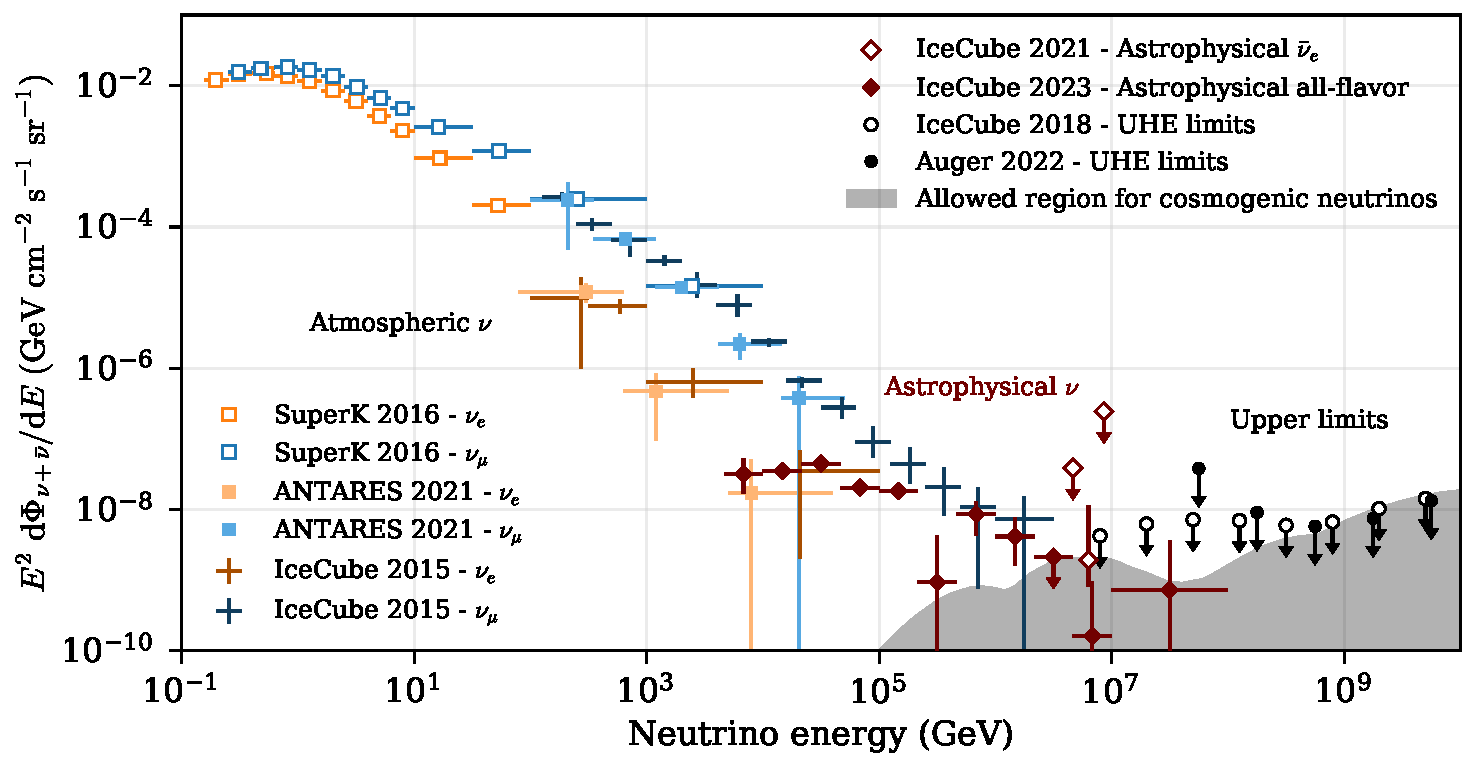
\includegraphics{./figures/nu_he/neutrino_spectrum_wide_231010.pdf}
    \labfig{nu_fluxes}
\end{figure}
The aforementioned sample of starting events, that uses outer layer of the detector as an active veto was used to find an evidence for astrophysical neutrinos was first observed by IceCube in 2013 \sidecite[-13.5cm]{Evidence_paper}. While subsequent analyses reinforced this discovery \sidecite[-12cm]{HESE4,HESE6}, different studies using various event samples revealed power-law indices spanning from \( E^{-2} \) to \( E^{-3} \), suggesting potential substructures within the flux \sidecite[-2.5cm]{diffusenumu,cscd_6yr,lars_globalfit,HESE7_sample,ESTES}. Although initial data hinted at these features, two recent independent IceCube studies confirmed a spectral break in the neutrino spectrum: hardening below 30 TeV and softening at higher energies, with a broken power law preferred over a single power law with more than \( 4\sigma \) significance \sidecite[-12cm]{globalfit_icrc,MESE_ICRC}. This spectral break offers key insights into the underlying astrophysical neutrino production mechanisms. \reffig{nu_fluxes} shows the most updated measurements for both atmospheric and astrphysical fluxes of neutrinos, along with limits at higher energies for cosmogenic neutrinos. 


%SuperK 2016 [243]; ANTARES 2021 [244]; IceCube 2015 νe [245]; IceCube 2015 νμ [246]; IceCube 2021 astrophysical ν ̄e (ν + ν flux derived from a single candidate event for the Glashow resonance) [247]; IceCube 2023 astrophysical all flavour [39]. The limits at the highest energies are taken from [248] (IceCube) and [249] (Auger).

\subsubsection*{Source Candidates}
\label{sec:sources_astro_nu}

One of the main goals of IceCube is to point back to these high-energy neutrino sources. Previous but also on-going studies that utilize various event samples attempt to find the population(s) of sources responsible for these high-energy neutrinos\sidecite[-4cm]{Naoko_ICRC}. Since gamma rays and neutrinos are produced together in the same environment through the processes discussed above, a simultaneous observation of gamma rays and neutrinos coming from the same source serves as a strong evidence of it being a neutrino source. In the general picture of \emph{multi-messenger astronomy}, the connection between different messengers can shed light in the physical properties of extreme astrophysical environments, and simultaneous observations are a key ingredient to achieve that. To facilitate this endeavor, IceCube issues \emph{a realtime alert} of neutrino events that are the most promising high-energy events \sidecite[-7cm]{realtime}, by sending out the possible direction and energy of the event to the astronomical community, so that they can further look for contemporary detections in different messengers.

Such an approach gave IceCube its first ever smoking gun signature of a neutrino emitter. The neutrino alert event IC170922A was found spatially coincident with the blazar TXS 0506+056 while it was flaring, with the flare established by multi-wavelength observations of the source, initiated by the neutrino alert \sidecite[-9.5cm]{txspaper}. An archival search found another neutrino flare, which further strengthened the case of TXS 0506+056 as a neutrino source; however, it was not accompanied by enhanced electromagnetic emission \sidecite[-9cm]{txspaper2} that poses a problem when modeling neutrino production in blazars \sidecite[-8cm]{Winter:2019hee}. In fact, a search for correlations between blazars and neutrino alert events using a catalog of blazars yielded no significant signal for any of them, which is compatible with a small fraction (< 1\%) of blazars being neutrino emitters \sidecite[-7.5cm]{cris_paper}. Nevertheless, AGN remain strong candidates for neutrino source, as there is strong evidence, at the $4.2\,\sigma$ levell, that the active galaxy NGC 1068 is a neutrino source \sidecite[-7cm]{ngc1068}.

Another proposed source class is \textbf{a Tidal Disruption Event (TDE)}. TDEs are transients that occur when a star passes close to a Supermassive Black Hole (SMBH) and gets disrupted by the tidal force due to the strong gravity. This creates a very bright electromagnetic flare that lasts for months. TDEs have been proposed as high-energy neutrino and ultra-high-energy cosmic ray sources \sidecite[-8.5cm]{Hayasaki_2021}. So far, three TDEs were found to be associated to IceCube neutrino events: the AT2019dsg to the IC191001A event \sidecite[-8.5cm]{Stein_2021}, the AT2019fdr to the IC200530A event \sidecite[-7.5cm]{simeon_tde}, and the AT2019aalc to the IC191119A event \sidecite[-6.5cm]{vanVelzen:2021zsm,}, making this source class relevant for population studies \sidecite[-5cm]{Winter:2022fpf}.

Gamma-ray bursts (GRBs) have long been considered prime candidates for cosmic-ray and associated neutrino production \sidecite[-5cm]{Murase:2014tsa,Kumar:2014upa,Zhang:2017moz,GRB_lumino}. Neutrino emission could theoretically occur at various stages of a GRB: during the pre-burst phase of the progenitor star \sidecite[-2.5cm]{Razzaque:2003uv}, the prompt gamma-ray emission phase \sidecite[-2cm]{Murase:2008sp}, and potentially in the afterglow \sidecite{Waxman:1999ai}. However, early investigations by IceCube showed no significant evidence of high-energy neutrinos linked to gamma-bright GRBs \sidecite{2012}. Further analyses strengthened these findings, indicating that GRBs likely contribute less than about 1\% to the observed diffuse neutrino flux \sidecite{IceCube:2017amx}. This constraint suggests that other source classes may play a larger role in the observed astrophysical neutrino fluxe. 

Another breakthrough occured recently when IceCube reported observation of a diffuse neutrino flux from the Galactic Plane with a $4.5\sigma$ significance \sidecite{icecube_milkyway}. This measurement was revolutionizing as due to location of the IceCube, Because the Galactic center is located in the Southern Sky, diffuse emission is expected to be concentrated in the Southern Sky. IceCube is located at the South Pole, so observations in the southern celestial sky are composed of events downgoing in the detector. Searches in this region are particularly difficult due to the large background of atmospheric muons. Thanks to machine learning techniques, used for careful reconnstruction of the cascade like event, it was possible to make use of a sample, which can improve signal-to-background ratio of these events significantly.


As mentioned above, associations with individual srcs have been established, but in terms of populations there are no conclusive results. The fractional contribution of the various src classes to the diffuse neutrino flux remains unknown.

\subsubsection{Flavour Composition}
\label{sec:flavor_theory}
As discussed before, neutrinos are produced via the decays of charged pions and muons, leading to the generation of only $\nu_e$ and $\nu_\mu$.

\marginnote{\begin{kaobox}
flavour composition, or alternatively called the flavour ratio, is described as a set of three numbers, $(f_e : f_\mu : f_\tau)$, often normalized so that $f_e + f_\mu + f_\tau = 1$, representing the fraction of each neutrino flavour in the astrophysical flux.
\end{kaobox}}

The flavour composition of neutrinos can significantly vary depending on the environments of high-energy neutrino sources. For instance, produced pions and muons may interact before decaying, thereby altering the expected neutrino ratios. This leads to several \textbf{source scenarios}, each resulting in different overall flavour compositions.

The scenario discussed in Section~\ref{sec:astro_nu} describes the \textbf{pion production scenario}, where the source environments are assumed to be sparse enough that the produced muons and pions do not interact before decaying. In this case, the expected flavour composition at the source would be $\nu_e:\nu_{\mu}:\nu_{\tau} = 1:2:0$.


In magnetic field environments, charged pions and muons from $pp$ and $p\gamma$ interactions can undergo significant synchrotron energy losses, around $(m_p/m_{\pi,\mu})^3 \sim 10^3$ times greater than for protons. Given their $\tau_\mu/\tau_{\pi^\pm} \sim 10^2$ times longer lifetimes \sidecite[-4cm]{PDG_2024}, muons are more likely to interact before decaying, rendering these sources opaque to muons and thus eliminating their contribution to the neutrino flux. In this \textbf{muon-damped scenario}, the source flavour composition shifts to $f_{\nu_e} : f_{\nu_\mu} : f_{\nu_\tau} = 0 : 1 : 0$ \sidecite[-2cm]{cite166,walter_muondamped,cite170}. Since the muon interaction probability increases with energy, a realistic model would show an energy-dependent shift in flavour composition from $1 : 2 : 0$ to $0 : 1 : 0$ over 1-2 decades in energy, expected around $\sim 100$ TeV for GRBs \sidecite{cite166}.

Additionally, in sources with dominant $p\gamma$ interactions and extremely strong magnetic fields, the \textbf{neutron-beam scenario} leads to a flavour composition of $f_{\nu_e} : f_{\nu_\mu} : f_{\nu_\tau} = 1 : 0 : 0$ \cite{flavour1}. Here, highly energetic neutrons are produced, either through processes like those in Equation~\ref{eq:direct_pion} or by photodisintegration of heavy cosmic-ray nuclei. For neutrons to decay via $n \rightarrow p + e^- + \bar{\nu}_e$, the source environment must be optically thin, as a result $\bar{\nu}_e$ are generally lower in energy compared to neutrinos from charged pion or muon decay. Strong magnetic fields are also needed to cool charged pions and muons through synchrotron losses, preventing their decays from contributing to the high-energy neutrino spectrum \sidecite{Hummer:2010vx}.

For sources with dominant $pp$ interactions at very high energies, heavier mesons such as charmed mesons can form. This \textbf{charm-production scenario} has a flavour composition of $f_{\nu_e} : f_{\nu_\mu} : f_{\nu_\tau} = 1 : 1 : 0$ \sidecite{prompt_tau}, similar to the production of prompt atmospheric neutrinos (see Section~\ref{sec:atm_nu}). Here, charmed $D$-meson decay produces equal amounts of $\nu_e$ and $\nu_\mu$, with tau neutrinos contributing about 5\%, which can be neglected. While heavier mesons could form, bottom mesons are produced at roughly 10 times lower rates than charmed mesons \sidecite{cite59}. This composition, $f_{\nu_e} : f_{\nu_\mu} : f_{\nu_\tau} = 1 : 1 : 0$, can also arise from energy-dependent secondary acceleration of muons and pions at the source \sidecite{cite168}.
\begin{figure}[h!]
    \caption[The measured and theoretically possible astrophysical neutrino flavour compositions at Earth]{The measured flavour composition of IceCube's high-energy starting events (HESE) is shown. The contours represent the $1\sigma$ and $2\sigma$ confidence intervals. Shaded regions indicate previously published results \cite{lars_globalfit,gary_paper}, which lacked direct sensitivity to the tau neutrino component. Expected flavour compositions for various astrophysical neutrino production mechanisms discussed in text marked on the figure. The dotted  gray line represents the theoretically allowed flavour ratios at Earth for different choices of source ratios, assuming standard mixing \cite{muon_damp}. Figure from \cite{Juliana_paper}}
    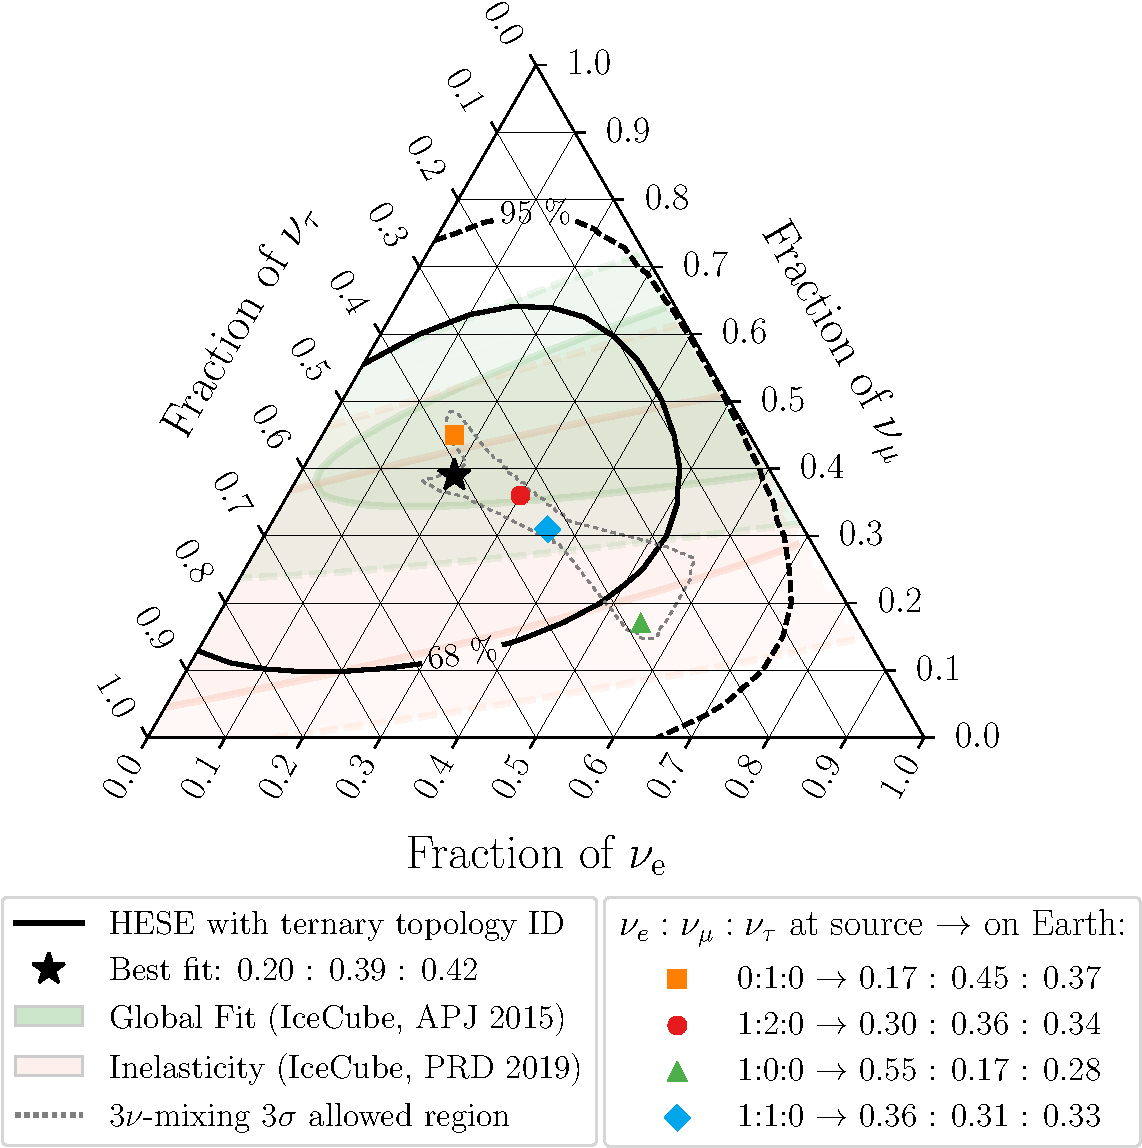
\includegraphics{./figures/nu_he/flavor_scan_7yr_steps21_inel_gf_source_shaded_serif_paper.pdf}
    \labfig{flav_triangle}
\end{figure}
In general, realistic sources likely exhibit varying flavour compositions that depend on energy and the source environment \sidecite{cite169}. These scenarios fit within a broader model that parameterizes flavour composition by the size and magnetic field of the acceleration region in the Hillas phase space \sidecite{cite170}, incorporating synchrotron cooling and high-energy processes to suggest a range of energy-dependent transitions among individual cases.

Due to neutrino oscillations, the flavour composition undergoes changes as neutrinos travel from source to observer. Astrophysical neutrinos are likely produced incoherently in the scenarios described above, possessing varying energies at different locations near the source and traversing cosmic distances before detection on Earth. Recall the transition probability for neutrino oscillations, where a neutrino from flavour eigenstate $\alpha$ can be measured in flavour eigenstate $\beta$ as expressed in Equation~\ref{eq:main_probability}:

\[
P(\nu_\alpha \to \nu_\beta) = |U_{\alpha j}| |U_{\beta j}| + 2 \text{Re}(U_{\alpha j} U_{\beta j} U_{\alpha k} U_{\beta k} e^{i \Delta m^2 L / 2E}),
\]

where separating diagonal and off-diagonal terms leads to:

\[
\langle P(\nu_\alpha \to \nu_\beta) \rangle = X |U_{\alpha j}|^2 |U_{\beta j}|^2.
\]

This result is independent of $\Delta m^2$, $E$, and $L$, meaning that the expected astrophysical neutrino flavour composition at Earth is fully determined by the emitted composition at the source and the mixing parameters $\theta_{12}, \theta_{23}, \theta_{13}$, and $\delta_{CP}$.Utilizing the current best-fit measurements detailed in Table~\reftab{mixing_parameters}, we can derive the measured flavour ratios for the various scenarios:

\begin{kaobox}
\centering
\textbf{Pion-production scenario:} $1 : 2 : 0 \rightarrow 0.31 : 0.35 : 0.34$\\ 
\textbf{Muon-damped scenario:} $0 : 1 : 0 \rightarrow 0.19 : 0.43 : 0.38$\\ 
\textbf{Neutron-beam scenario:} $1 : 0 : 0 \rightarrow 0.55 : 0.19 : 0.26 $\\
\textbf{Charm-production scenario:} $1 : 1 : 0 \rightarrow 0.37 : 0.31 : 0.32$\\
\end{kaobox}

Despite the vast range of conceivable neutrino flavour compositions associated with cosmic rays, the theoretically detectable compositions at Earth are confined to a narrow phase space \sidecite{muon_damp}, as shown by the dotted grey lines around various colorful points in \reffig{flav_triangle}. Moreover, this region encompasses the uncertainties in the mixing parameters at the $3\sigma$ confidence level. This result has two notable implications: first, the limited phase space of detectable flavour compositions at Earth suggests that high-precision measurements are crucial for excluding specific source models. Second, any production scenario predicts that the detectable astrophysical tau-neutrino fraction at Earth will be significantly greater than zero.

This makes flavour measurement of astrophysical neutrinos an intriguing probe for examining source contributions to the diffuse neutrino spectrum. Several studies within IceCube have attempted to measure this flavour ratio, as shown in \reffig{flav_triangle}. As emphasized earlier, and visible in the figure, the main factor in measuring flavour composition is identifying tau neutrino events, since regardless of the favored scenario, a non-zero tau fraction is expected. The flavour triangle in \reffig{flav_triangle} illustrates three measurement using three distinct IceCube samples \sidecite[-4cm]{lars_globalfit,gary_paper,Juliana_paper}, where only the most recent measurements, which used the all-flavour starting event sample \cite{Juliana_paper}, achieved the first-ever non-zero $\nu_\tau$ fraction by identifying two tau neutrino candidates in IceCube. A subsequent study used a \emph{convolutional neural network (CNN)} approach to search for $\nu_\tau$ events and found 7 $\nu_\tau$ candidates in IceCube data \sidecite[-2cm]{CNN_tau}, ruling out the absence of an astrophysical $\nu_\tau$ flux at the $5\sigma$ level. The aim of this thesis is to measure the neutrino flavours in astrophysical srcs, by refining these measurements, hence provide crucial insights into the flavour composition of the diffuse neutrino spectrum.



